\documentclass[12pt]{article}
\usepackage[spanish]{babel}
\usepackage[utf8]{inputenc}
\usepackage{amsmath}
\usepackage{listings}
\usepackage[usenames]{color}
\definecolor{gray97}{gray}{.97}
\definecolor{gray75}{gray}{.75}
\definecolor{gray45}{gray}{.45}
\definecolor{azul1}{RGB}{141,198,163}
\definecolor{azul2}{RGB}{24,107,122}
\definecolor{verde1}{RGB}{44,186,34}
\usepackage{graphicx}
\usepackage{caption}
\usepackage{subcaption}
\usepackage{textcomp}
\lstset{
        frame=Ltb,
        framerule=1pt,
        framextopmargin=3pt,
        framexbottommargin=3pt,
        framexleftmargin=0.6cm,
        framesep=0pt,
        rulesep=.4pt,
		backgroundcolor=\color{gray97},
		rulesepcolor=,
        tabsize=4,
        rulecolor=\color[RGB]{106, 182, 217}, %AZUL
        upquote=true,
        aboveskip={1.5\baselineskip}, %despues de la linea de texto
        columns=fixed,
        showstringspaces=false,
        extendedchars=true,
        breaklines=true,
        prebreak = \raisebox{0ex}[0ex][0ex]{\ensuremath{\hookleftarrow}},
        showtabs=false,
        showspaces=false,
        showstringspaces=false,
        basicstyle=\scriptsize\ttfamily\color[RGB]{39, 100, 46}, %Numeros de lineas, simbolos, puntos y coma y demas
        identifierstyle=\ttfamily\color[RGB]{56, 140, 189}, %variables
        commentstyle=\color[RGB]{62, 179, 101}, %comentarios
        stringstyle=\color[RGB]{247, 165, 42}, %impresiones
        keywordstyle=\bfseries\color[RGB]{237, 118, 150}, %funciones
        %
		numbers=left,
		numbersep=5pt,
		numberstyle=\tiny,
		numberfirstline = false,
		breaklines=true,
		}
\usepackage{graphicx}
\usepackage[colorinlistoftodos]{todonotes}
\usepackage{natbib} %citas bibliograficas estilo APA :p
\usepackage{eso-pic}
\usepackage{avant}
\usepackage[top=2cm,bottom=2cm,left=2.5cm,right=3cm,headsep=8pt,a4paper]{geometry}
\usepackage{fancyhdr}
\pagestyle{fancy}
\fancyhf{}
%\fancyhead[LE,RO]{}
\fancyhead[RE,LO]{Procesamiento de Señales II}
\fancyfoot[CE,CO]{\leftmark}
\fancyfoot[LE,RO]{\thepage}
\renewcommand{\headrulewidth}{2pt}
\renewcommand{\footrulewidth}{1pt}
\usepackage{hyperref}
\usepackage{tabu}
\usepackage{array}
\usepackage{multirow}
\usepackage{amssymb}
\usepackage{makeidx}
\graphicspath{ {images/} }
\usepackage{wrapfig}
\usepackage{enumerate}
\usepackage{amsmath,tikz}
\usetikzlibrary{matrix}
\usepackage{steinmetz}
\newcommand*{\horzbar}{\rule[0.05ex]{2.5ex}{0.5pt}}
\usepackage{calc}
\date{\today}


\begin{document}

\begin{titlepage}
\newcommand{\HRule}{\rule{\linewidth}{0.5mm}} 
\center
\textsc{\LARGE  Benemérita Universidad \\[0.2cm] Autónoma de Puebla}\\[1.5cm] 

\includegraphics[width=4cm]{escudo.jpg}\\[1cm]
\textsc{\Large Facultad de Ciencias de la Electrónica}\\[0.5cm] 
\textsc{\large Licenciatura en Electrónica}\\[0.5cm]
\HRule \\[0.4cm]
{ \huge \bfseries Segundo Examen Parcial }\\[0.4cm] 
\HRule \\[1.5cm]
\begin{minipage}{\textwidth}
\center 

\emph{Profesor:} \\
Fernando López Marcos \\[1cm]

\begin{tabular}{ll}
\emph{Alumnos:} & \emph{Número de Matrícula:}\\
Hanan Ronaldo Quispe Condori  & 555010653 \\
Erick Sandro Niño García & 201631150\\
Carlos Alfredo Vega Aguilar & 201632131 \\
\end{tabular}
\end{minipage}\\[2cm]
\today
\end{titlepage}

%\newpage
%~\vfill
%\thispagestyle{empty}
%\begin{figure}[hbtp]


%\includegraphics[width=4cm]{IMAGENES/motordc}
%\end{figure}
%\noindent \textsc{Trabajo Encargado: Problemas en MatLab \\ Máquinas Eléctricas \\ Universidad Nacional de San Antonio abad del Cusco}\\
%noindent \textsc{Ingeniería Electrónica }\\
%\noindent \textit{Tercera revisión, \today}

%\tableofcontents indice bloqueado xD

\newpage

\section{Planteamiento del Problema}
Se realizó la adquisición de una señal de voz, pero debido a que el procedimiento fue realizado
en un ambiente exterior, ésta posee una fuerte contaminación proveniente de fuentes no
deseadas. Se realizó un estudio breve de la naturaleza del ruido contenido en esta señal y la
mayor parte se encuentra concentrado en frecuencias superiores a la señal de voz.
\begin{enumerate}
    \item Plantee un filtro analógico que permita acondicionar la señal de voz. Las características de diseño (tipo, orden del filtro, frecuencias de corte, etc.) serán seleccionadas a su criterio, pero deben ser las idóneas para la tarea que se está encomendando. Puede valerse de Filter Design Tool para esta labor.
    \begin{enumerate}
        \item Describa la estructura del filtro y los componentes necesarios.
        \item Obtenga la respuesta en frecuencia del filtro analógico diseñado y verifique que cumpla con las características de diseño planteadas con anterioridad.
    \end{enumerate}
    \item Considerando una frecuencia de muestreo de 44100 Hz, repita el procedimiento del paso 1, pero esta vez plantee un filtro digital que permita acondicionar dicha señal. Nuevamente las características del filtro serán diseñadas a criterio propio, cumpliendo con los requerimientos planteados anteriormente. Puede utilizar fdatool para este ejercicio.
    \begin{enumerate}
        \item Describa la estructura del filtro digital seleccionado.
        \item Obtenga la respuesta en frecuencia del filtro digital diseñado y verifique que cumpla con las características de diseño planteadas con anterioridad. 
    \end{enumerate}
\end{enumerate}
\section{Solución de Problema}
\begin{enumerate}
    \item 
    \begin{enumerate}
        \item Valiéndose de la herramienta de diseño de filtros de Texas Instruments, Filter Design Tool, y considerando las siguientes carácterísticas de diseño:
        \\
        Filtro Butterworth pasa bajas de órden 5 y topología Sallen - Key.
        $$f_{corte} = 3 kHz$$
        $$f_{stopband} = 8 kHz$$
        Se decidieron las anteriores características ya que según algunas investigaciones, la voz se encuentra en el rango de frecuencias entre 250 y 3000 Hz por lo que un filtro con frecuencia de corte a los 3 kHz es lo más óptimo. Se decidió agregar también, una frecuencia para la banda de rechazo de 8 kHz debido a que algunos fonemas de la voz humana se encuentran situados entre los 4000 y 8000 Hz, entonces se consideró apto que el filtro comenzara a rechazar señales a partir de los 3 kHz y tuviera su completa filtración a los 8 kHz. 
        \\
        El orden del filtro fue sugerido por el modo automático del FDT, pero al ver que el circuito consistía en 3 amplificadores operacionales en cascada, se buscó hacerlo de un orden menor para intentar que el filtro esté compuesto de solo un OpAmp, pero no se consiguió si no hasta reducirlo a un segundo orden. Después de analizar las gráficas del comportamiento del filtro de segundo orden y quinto orden, se optó por utilizar este último debido a su nivel de atenuación en la frecuencia de banda de rechazo.
        \\
        En las siguientes imágenes se muestra el comparativo mencionado anteriormente que además, muestra porqué se eligió un filtro Butterworth por encima de un Chebyshev:
        \\
        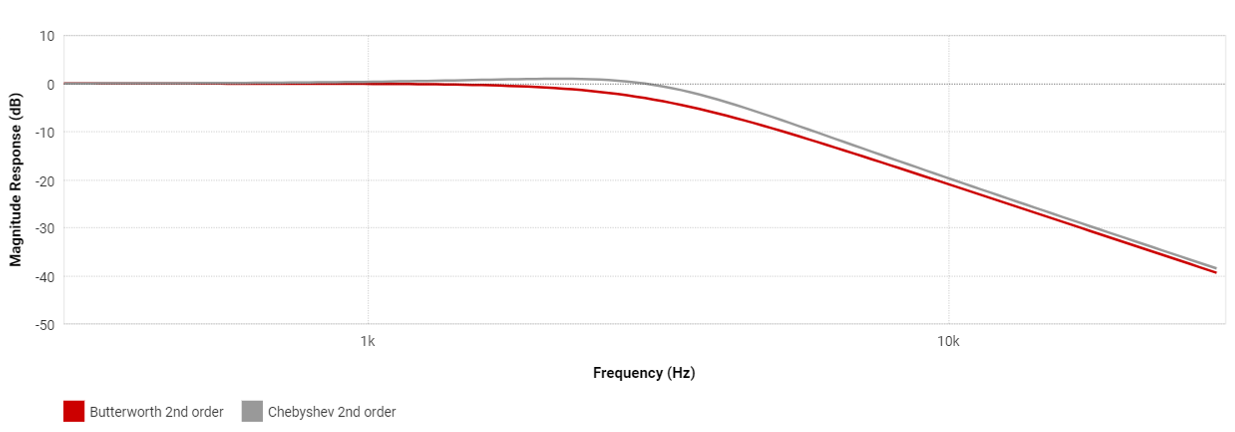
\includegraphics[scale=0.50]{But_vs_Cheb_2ord.png}
        \\
        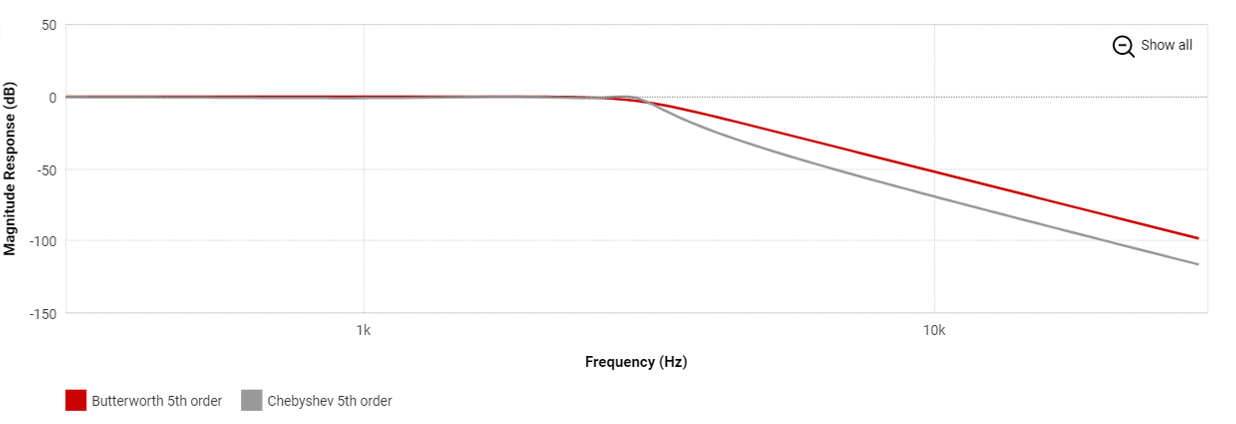
\includegraphics[scale=0.50]{But_vs_Cheb_5ord.png}
        \\
        La pendiente de la banda de transición en el filtro de segundo orden es muy similar para el Butterworth y para Chebyshev. En cambio, para el filtro de orden 5 la diferencia es más notable teniendo una pendiente más inclinada el Chebyshev pero teniendo un pequeño lóbulo o rizo en la rodilla de la gráfica. Debido a que se desconoce que tan estricta debe ser la filtración de la señal, se optó por un Butterworth ya que su pendiente es muy buena y no tiene rizos en la banda de paso ni en rechazo.
        \\
        \item Se replicó el diagrama circuital que arrojó Filter Design Tool para simularlo en TopSpice para comprobar su funcionaiento, los resultados fueron los siguientes:
        \\
        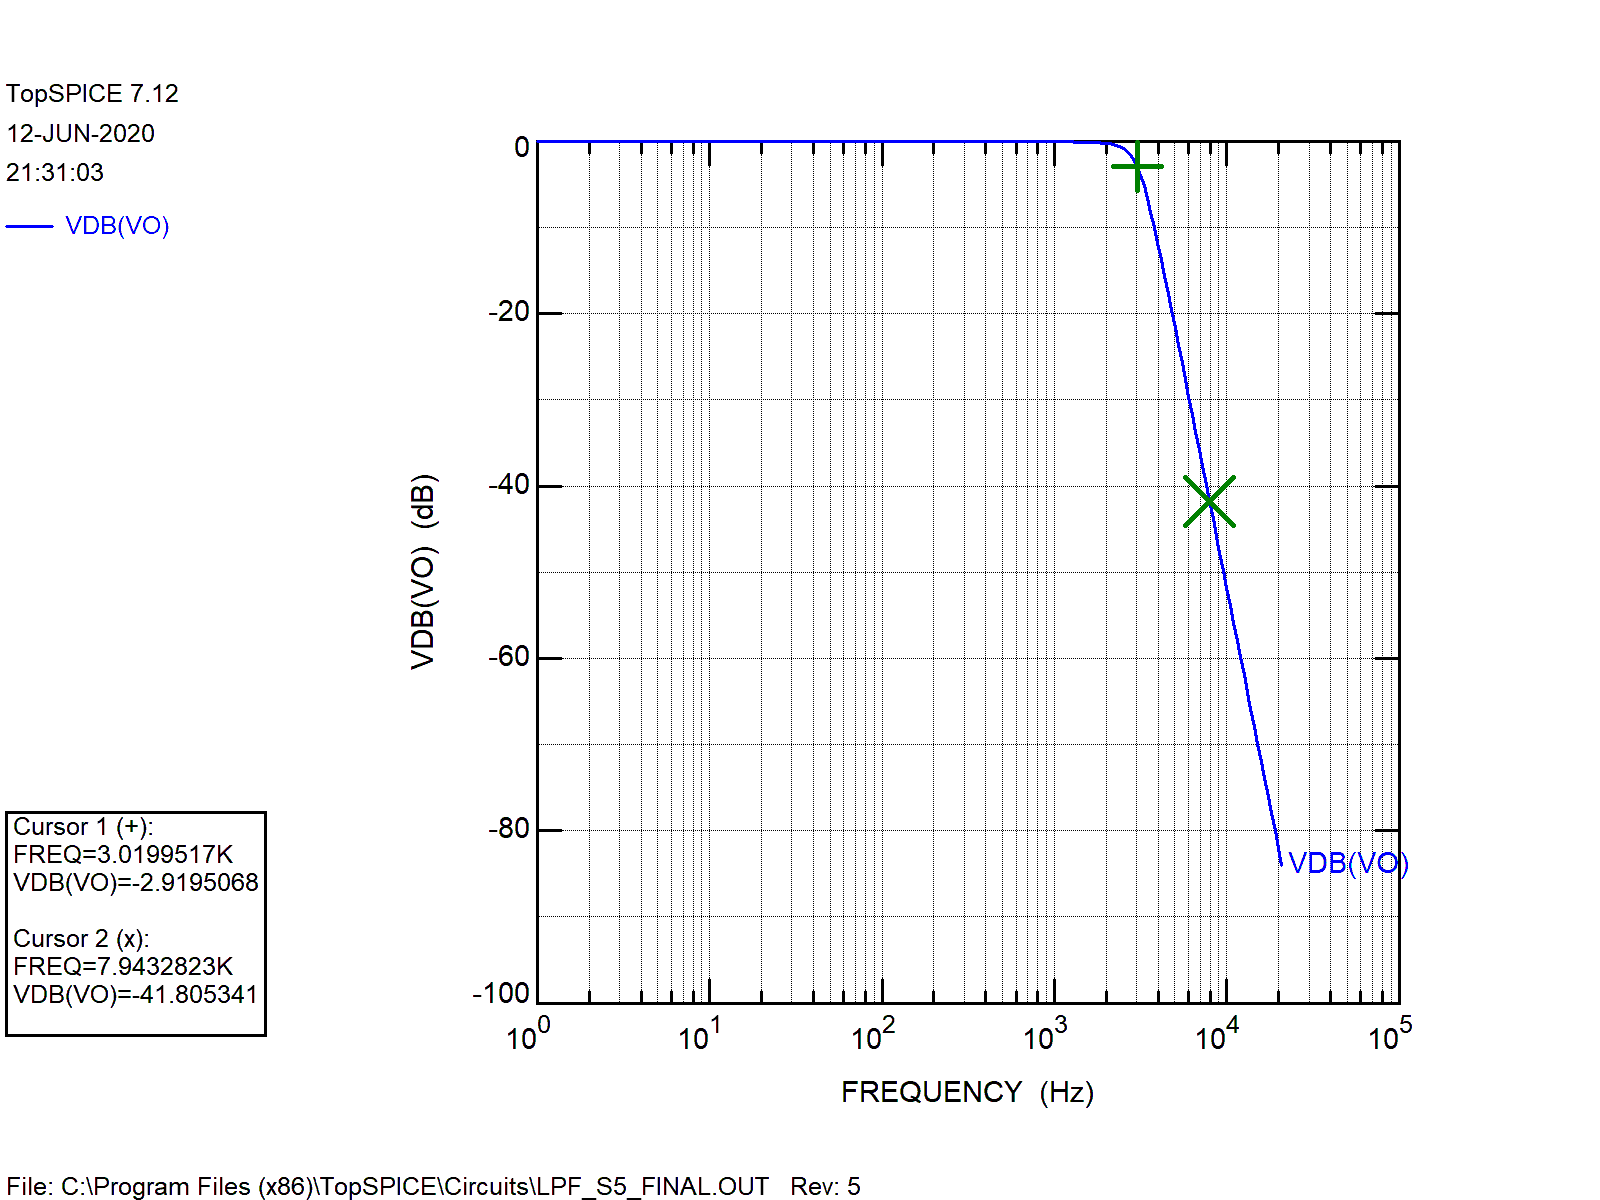
\includegraphics[scale=0.20]{Bode_Filtro_Anal.png}
        \\
        \\
        Se observa que en la frecuencia de corte se obtuvieron prácticamente los -3dB, valor ideal y muy buscado en cuanto a filtros respecta, además, a la frecuencia de 8 kHz se obtuvo una atenuación de -41 dB, esto significa que incluso desde frecuencias un tanto inferiores a esta, el filtro ya está rechazando señales ubicadas en estas frecuencias. Recordando que se decidió este parámetro para la banda de rechazo ya que algunos fonemas están ubicados a dichas frecuencias, pero si la grabación tuviese ruido cuya frecuencia se encuentre por debajo de 8Khz, este sería rechazado en su mayoría. 
    \end{enumerate}
    \item 
    \begin{enumerate}
        \item Se especifico que la aplicación del filtro será para el tratamiento de audio, por lo que se eligio usar un filtro IIR eliptico por su bajo coste computacional a la hora de ejecutarlo, al usar fdatool para el diseño del filtro se obtuvieron los siguientes coeficientes.
        \lstinputlisting[language=Matlab]{coeff_orden_5.fcf}
        La estructura del filtro corresponde a la forma directa número 2
        con tres secciones de orden 5 cada una, esto quiere decir que cada sección tendra 5 atrasos $z^{-1}$ en su extructura. Cada sección estara conectada a la siguiente en cascada, los coeficientes de esta estructura se podrán encontrar usando la función $sos2tf$, estos tendrán los siguientes valores. 
        \lstinputlisting[language=Matlab]{diary}
        \item La respuesta en frecuencia del filtro se obtendrá usando la función $freqz $ de MATLAB, como se indicá en el siguiente script.
        \lstinputlisting[language=Matlab]{finale.m}
        En el script se ingresaron las matrices obtenidas usando fdatool, una vez convertida la matriz $SOS$ a función de transferencia, finalmente se puede usar la $freqz$ como se indicó anteriormente.
        La repuesta en frecuencia del filtro se muestra en la figura (\ref{fig:freq_resp}).
        
        \begin{figure}[h]    
            \centering
            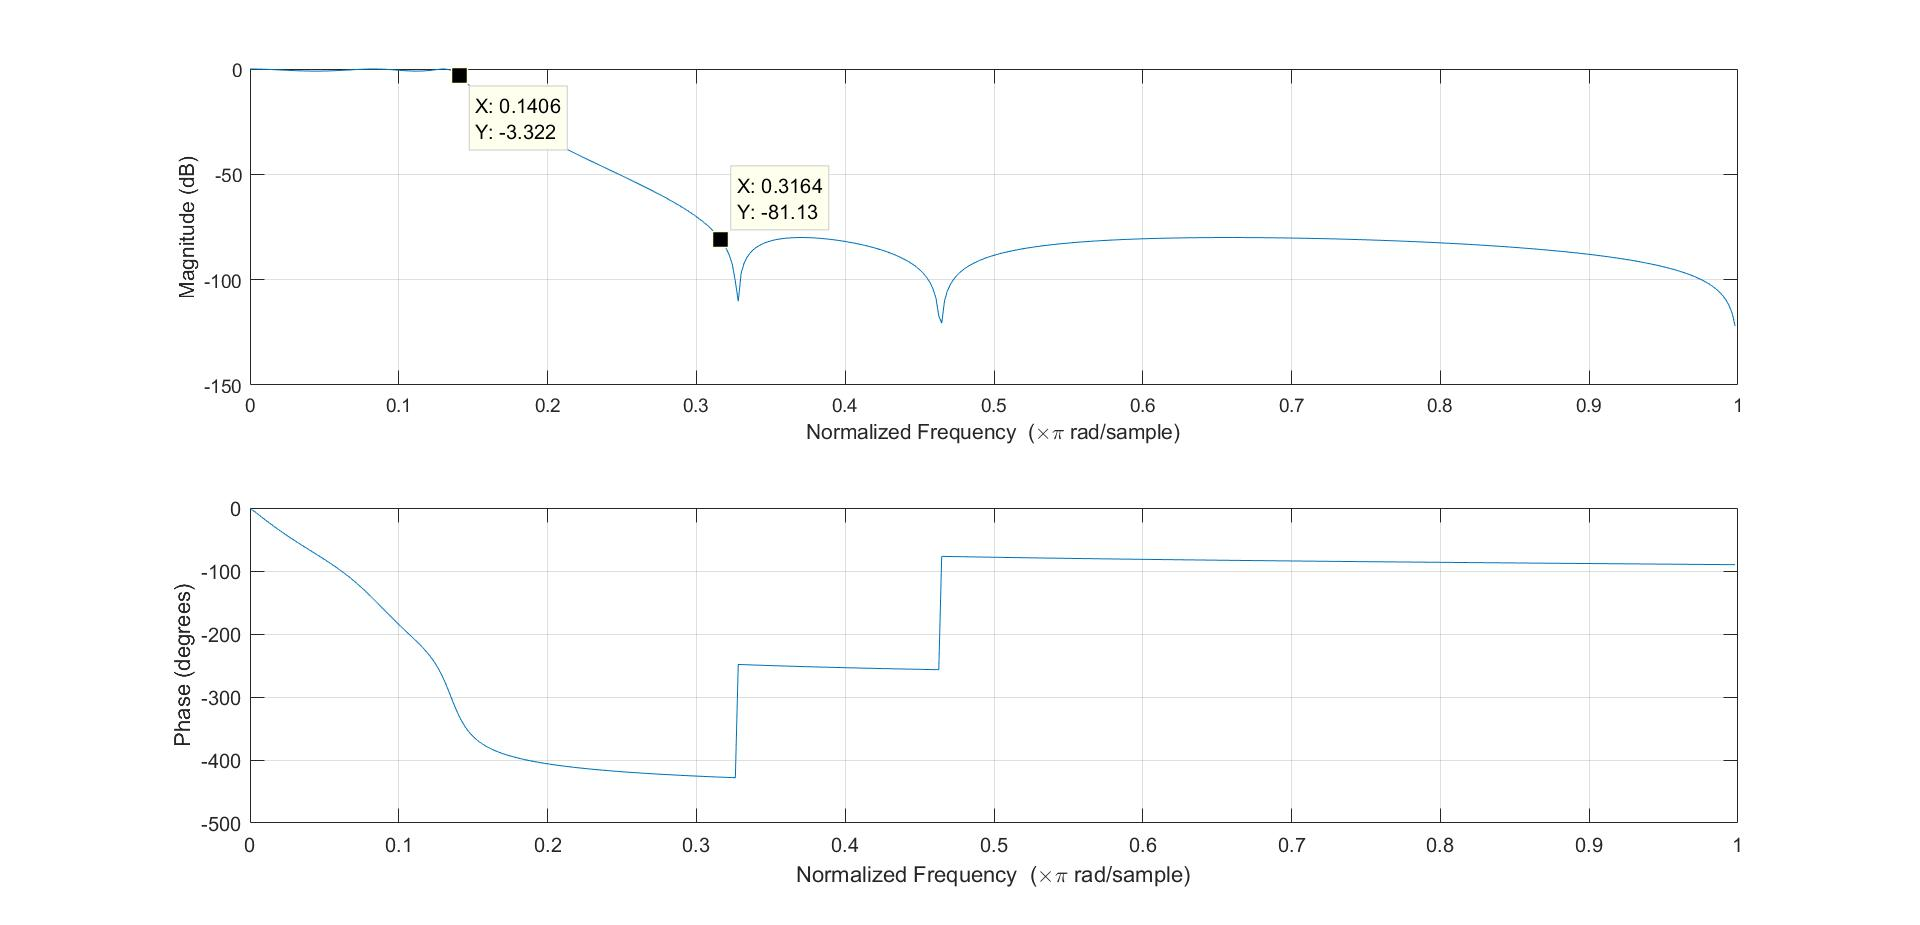
\includegraphics[width=15cm]{iir_filter.jpg}
            \caption{Respuesta en Frecuencia del Filtro.}
            \label{fig:freq_resp}
        \end{figure}
        
        En la figura (\ref{fig:freq_resp}) se marcaron 2 puntos de interes, el primero marca el lugar aproximado de la frecuencia de corte del filtro, la cual como requiere la aplicacion de filtrado de una señal de voz, se indicó en los parametros de diseño del filtro para que se encuentre en los $3kHz$, el punto marcado indica $0.1406$ lo cual al estar en frecuencia normalizada, expresado en $Hz$ es, $0.1406*22500=3163.5Hz$, este es un valor muy cercano a la frecuencia de corte especificada, por lo cual podemos asegurar que se cumple con esta característica de diseño.
        \\
        El siguiente punto de interes se encuentra en la frecuencia de rechazo $8kHz$. El punto marcado nos indica $0.3164$ lo cual al estar en frecuencia normalizada, expresado en $Hz$ es, $0.3164*22500=7119Hz$, en este punto la atenuación obtenida fue de $-81Db$, este valor como en el caso anterior es tambien cercano a lo especificado a la hora de diseñar el filtro.
        \\
        Se puede concluir que se cumplen con las características de diseño planteadas para esta aplicación.
    \end{enumerate}
\end{enumerate}
\end{document}
